
%%%%%%%%%%%%%%%%%%%%%%% file typeinst.tex %%%%%%%%%%%%%%%%%%%%%%%%%
%
% This is the LaTeX source for the instructions to authors using
% the LaTeX document class 'llncs.cls' for contributions to
% the Lecture Notes in Computer Sciences series.
% http://www.springer.com/lncs       Springer Heidelberg 2006/05/04
%
% It may be used as a template for your own input - copy it
% to a new file with a new name and use it as the basis
% for your article.
%
% NB: the document class 'llncs' has its own and detailed documentation, see
% ftp://ftp.springer.de/data/pubftp/pub/tex/latex/llncs/latex2e/llncsdoc.pdf
%
%%%%%%%%%%%%%%%%%%%%%%%%%%%%%%%%%%%%%%%%%%%%%%%%%%%%%%%%%%%%%%%%%%%

\documentclass[runningheads,a4paper]{llncs}
%\documentclass{report}

\usepackage[utf8]{inputenc}

\usepackage{natbib}
\bibliographystyle{apalike-cs}

\usepackage{amssymb}
\setcounter{tocdepth}{3}
\usepackage{graphicx}


% nastavení pisma a češtiny
\usepackage{lmodern}
\usepackage[T1]{fontenc}
%\usepackage[cp1250]{inputenc}
%\usepackage[czech]{babel}	

%Math
\usepackage{amsmath}


%Matlab
\usepackage[numbered]{mcode}

%code
\usepackage{listings}
\usepackage{textcomp}

\lstdefinestyle{Python}{
  language=Python,
  numbers=left,
  stepnumber=1,
  numbersep=10pt,
  tabsize=4,
  showspaces=false,
  showstringspaces=false
}

\lstdefinestyle{R}{
  language=R,
  numbers=left,
  stepnumber=1,
  numbersep=10pt,
  tabsize=4,
  showspaces=false,
  showstringspaces=false
}

%csv handling
\usepackage{csvsimple}

%H option for pictures
\usepackage{float}

% tables with merged 
\usepackage{multirow}

\usepackage{url}
\urldef{\mailsa}\path|{alfred.hofmann, ursula.barth, ingrid.haas, frank.holzwarth,|
\urldef{\mailsb}\path|anna.kramer, leonie.kunz, christine.reiss, nicole.sator,|
\urldef{\mailsc}\path|erika.siebert-cole, peter.strasser, lncs}@springer.com|    
\newcommand{\keywords}[1]{\par\addvspace\baselineskip
\noindent\keywordname\enspace\ignorespaces#1}

%subsubsection with new line
\makeatletter
\renewcommand\subsubsection{\@startsection{subsubsection}{3}{\z@}%
                       {-18\p@ \@plus -4\p@ \@minus -4\p@}%
                       {4\p@ \@plus 2\p@ \@minus 2\p@}%
                       {\normalfont\normalsize\bfseries\boldmath
                        \rightskip=\z@ \@plus 8em\pretolerance=10000 }}
\renewcommand\paragraph{\@startsection{paragraph}{4}{\z@}%
                       {-12\p@ \@plus -4\p@ \@minus -4\p@}%
                       {2\p@ \@plus 1\p@ \@minus 1\p@}%
                       {\normalfont\normalsize\itshape
                        \rightskip=\z@ \@plus 8em\pretolerance=10000 }}
\makeatother

\begin{document}

\mainmatter 

\title{Machine Learning A-Z}

\titlerunning{Machine Learning A-Z}

\author{Obrusník Vít}

\institute{CTU - Faculty of electrical engineering}

\authorrunning{Obrusník Vít}

\toctitle{}
\tocauthor{{}}

\maketitle

\begin{abstract}
This document summarizes Machine Learning A-Z course available at Udemy. \url{https://www.udemy.com/machinelearning/learn/v4/overview}. Authors are Kirill Eremenko and Hadelin de Ponteves.

All concepts are shown in Python and R. Course provides the students with code templates which are included in this document.

Every section has a dataset to train and test the model.
\end{abstract}

\medskip

\begingroup
\let\clearpage\relax
\tableofcontents
\addcontentsline{toc}{section}{Introduction}
\endgroup

\medskip
\medskip

\section{Preprocessing}
First of all we need to prepare our dataset. We can encounter several problems. Then we want to split the dataset.

\subsection{Problems with datasets}
\begin{enumerate}
\item Missing data

There might be some columns missing in the dataset. In that case our models won't work. We can either delete the incomplete rows or we can replace the missing data with average values. 

\item Categorical data

Some parameters (e.g. City['Madrid', 'Barcelano', 'Sevilla']) need to be replaced with integer values (e.g. City[1, 2, 3]). We need to focus on not to fall into \textbf{Dummy Variable Trap}. More information: \url{http://www.algosome.com/articles/dummy-variable-trap-regression.html}

\item Splitting the dataset into training set and test set

We usually train the model on 80\% of the dataset and test it on 20\%.

\item Feature scaling

We might want to scale the data to have normalized magnitudes. This is not always necessary and depends on the method/library. All the methods that use Euclidian distance are dependent on Feature scaled dataset.
\end{enumerate}

\subsection{Code template in Python}
Note that some parts of the code might be omitted.

\lstset{basicstyle=\tiny,style=Python}
\lstinputlisting[style=Python]{code/datapreprocessingtemplate.py}

\subsection{Code template in R}
Note that some parts of the code might be omitted.

\lstset{basicstyle=\tiny,style=R}
\lstinputlisting[style=R]{code/datapreprocessingtemplate.R}

\newpage

\section{Regression}

Regression is a statistical method of predicting the value of \textbf{dependent variable (DV)} based on values of \textbf{independent variable(s) (IVs)}. More information here \url{https://en.wikipedia.org/wiki/Regression_analysis}.

\subsection{Regression code template in Python}

\lstinputlisting[style=Python]{code/regression_template.py}

\subsection{Regression code template in R}

\lstinputlisting[style=R]{code/regression_template.R}

\subsection{Simple Linear Regression}

\textbf{Problem:} Our dataset contains years of experience and salary. We want to fit the model to recommend the salary based on years of experience. 

\csvautotabular{csv/Salary_Data.csv}

Simple Linear Regression is the easiest model following the equation

\begin{equation}
y = b_1 * x + b_0
\end{equation}

where $y$ is the dependent variable which we are interested in (salary) and $x$ is the independent variable (years of experience).

In order to use Linear Regression we simply replace comment from the template with the following code in Python

\lstset{basicstyle=\large,style=R}
\lstinputlisting[style=Python, linerange=25-28]{code/simple_linear_regression.py} 


And in R we use the following code to fit the Simple Linear Model

\lstset{basicstyle=\large,style=R}
\lstinputlisting[style=R, linerange=18-20]{code/simple_linear_regression.R} 


Results are following.

\begin{figure}[H]
\centering
\begin{center}
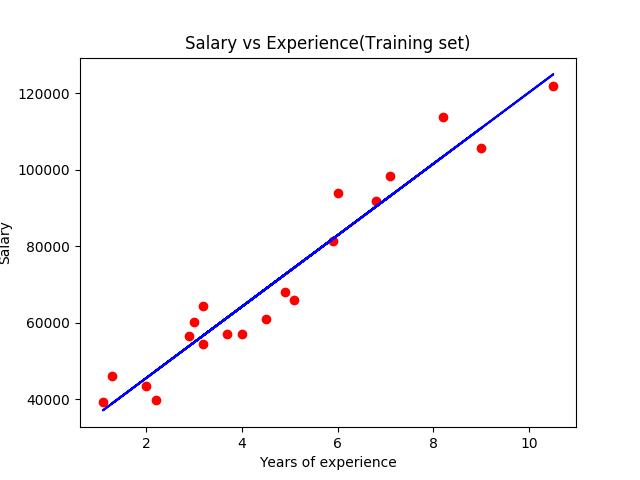
\includegraphics[scale=0.6]{pics/simple_linear_regression_python}
\label{uloha1:pic1}
\caption{Simple Linear regression in Python} 
\end{center}
\end{figure}



\subsection{Multiple Linear Regression}

\textbf{Problem:} We want to predict how profitable will the company be when we know its spending in R\&D, Advertisement and Administration. We have a dataset containing 50 startups, their country and their spending to train and test the model. This is the sample of the dataset:

%\csvautotabular{csv/Startups.csv}


Multiple Linear Regression follows this equation
\begin{equation}
y = b_1 * x_1 + b_2 * x_2 + \dots + b_n * x_n + b_0
\end{equation}

where $y$ is the dependent variable which we are interested in (profit) and $x_i$ is the independent variable (spending).

\subsubsection{Assumptions of Linear Regression}
There are several assumptions of Linear Regression:
\begin{itemize}
\item Linearity
\item Homoscedasticity

In statistics, a sequence or a vector of random variables is homoscedastic if all random variables in the sequence or vector have the same finite variance.

\item Multivariable normality

More information: \url{https://en.wikipedia.org/wiki/Multivariate_normal_distribution}
\item Independence of errors

Error values are statistically independent.
\item Lack of multicollinearity

Multicollinearity in regression occurs when predictor variables (independent variables) in the regression model are more highly correlated with other predictor variables than with the dependent variable.
More information: \url{http://www.researchconsultation.com/multicollinearity-multiple-regression.asp}
\end{itemize}

\subsubsection{5 methods of building models}

There are some methods to create predicting model. I am listing a few of them.
\begin{enumerate}
\item All-in (fit the model with all the independent variable)
\item Backward Elimination
\item Forward Selection
\item Bidirectional Elimination
\item Score comparison (fit the models with all possible combinations of independent variables and compare them)
\end{enumerate}

\subsubsection{Backward elimination}
While building a model we might want to get rid of some IVs. Some IVs usually don't have significant impact on the results. Backward elimination is an algorithm that can help us choose only significant variables.

\begin{enumerate}
\item Select a significance level to stay in the model (e.g. SL = 0.05)
\item Fit the full model with all possible predictors
\item Consider the predictor with the highest P-value. If P > SL, go to step 4, otherwise \textbf{Model is ready}
\item Remove the predictor
\item Fit the model without this variable
\end{enumerate}

\subsubsection{Forward Selection}

\begin{enumerate}
\item Select a significance level to stay in the model (e.g. SL = 0.05)

\item Fil all simple regression models $y ~ x_i$ Select the one with the lowest P-value

\item Keep this variable and fit all possible models with one extra predictor added to the one(s) you already have

\item Consider the predictor with the lowest P-value. If P < SL go to step 3. Otherwise \textbf{Your model is ready}
\end{enumerate}

\subsubsection{Bidirectional elimination}

\begin{enumerate}
\item Select a significance level to enter and to stay in the model (e.g. SLEnter = 0.05, SLStay = 0.05)

\item Perform the next step of Forward Selection (new variables must have P < SLEnter to enter)

\item Perform ALL steps of Backward Elimination (old variables must have P < SLStay to stay). 

\item No new variables can enter and no old variables can exit. \textbf{Your model is ready}
\end{enumerate}

\subsubsection{Code}
\bigskip
The following code implements Multiple Linear Regression in Python.

\lstinputlisting[style=Python, linerange=35-38]{code/multiple_linear_regression.py} 

\lstset{basicstyle=\tiny,style=Python}

The following code implements Backward elimination in Python. The method called \verb|summary()| is used to display all the P-values of Independent Variables. Then we choose the one with the biggest P-value, remove it and fit the modle again.
\lstinputlisting[style=Python, linerange=43-60]{code/multiple_linear_regression_be.py} 

\begin{figure}[H]
\centering
\begin{center}
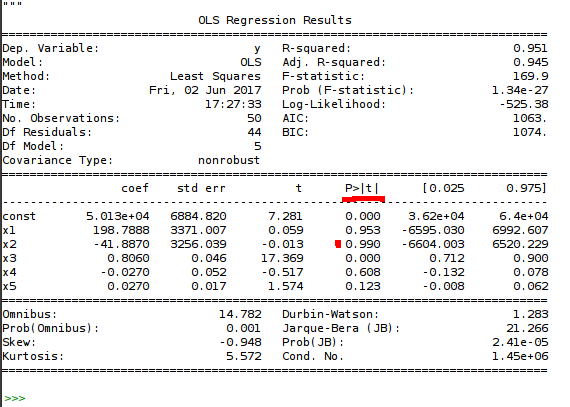
\includegraphics[scale=0.6]{pics/multiple_linear_regression_summary}
\label{uloha1:pic1}
\caption{Calling summary function in Python. We choose the variable with biggest P-value and remove it.} 
\end{center}
\end{figure}



The following code implements Multiple Linear Regression in R.

\lstset{basicstyle=\large}
\lstinputlisting[style=R, linerange=23-25]{code/multiple_linear_regression.R}
 
The following code implements Backward elimination in R.
\lstset{basicstyle=\tiny,style=R}

\lstinputlisting[style=R, linerange=30-46]{code/multiple_linear_regression_be.R} 


\subsection{Polynomial Regression}

\textbf{Problem:} We have a set of job positions and their according salaries. We want to train the model to propose the best salary for new empleyees. 

Polynomial regression is the first \textbf{nonlinear} model.

\csvautotabular{csv/Position_Salaries.csv}

\bigskip
Polynomial Regression follows this equation
\begin{equation}
y = b_1 * x_1^1 + b_2 * x_1^2 + \dots + b_n * x_n^n + b_0
\end{equation}

\lstset{basicstyle=\large}

The following code implements the Polynomial regressor in Python
\lstinputlisting[style=Python, linerange=28-34]{code/polynomial_regression.py} 


The following code implements the Polynomial regressor in R
\lstinputlisting[style=R, linerange=23-28]{code/polynomial_regression.R} 



The following picture shows visualisation of train model and real data (dots). Model is fitted by polynomial of 5th degree.

\begin{figure}[H]
\centering
\begin{center}
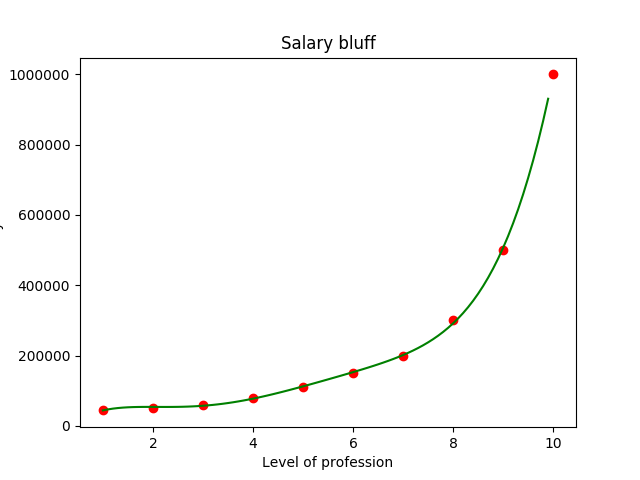
\includegraphics[scale=0.6]{pics/polynomial_regression_python}
\label{uloha1:pic1}
\caption{Polynomialregression in Python} 
\end{center}
\end{figure}

\subsection{Support Vector Regression (SVR)}

\textbf{Problem:} The same as in Polynomial regression. 

SVR is the second \textbf{nonlinear} model. SVR model from \verb|sklearn| Python library requires the dataset to be scaled in preprocessing.

The following code implements Support Vector Regressor in Python 

\lstinputlisting[style=Python, linerange=24-27]{code/svr.py} 

\textit{Kernel} is the method used by the predictor. \textit{RBF} means \textit{Radial Basis function kernel}. More information here: \url{https://en.wikipedia.org/wiki/Kernel_method}


\begin{figure}[H]
\centering
\begin{center}
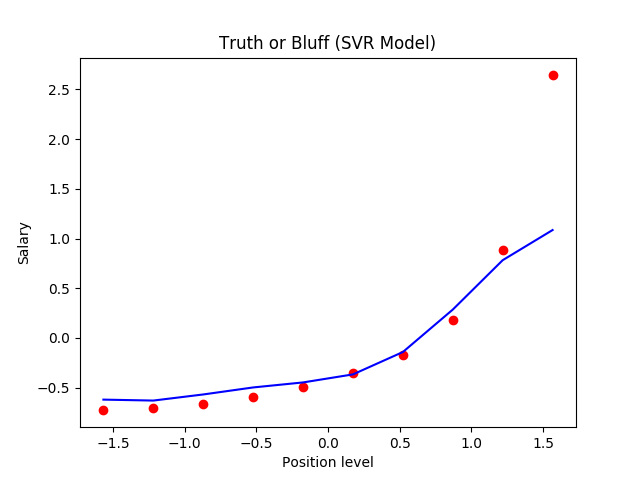
\includegraphics[scale=0.8]{pics/svr_python}
\label{uloha1:pic1}
\caption{Support Vector regression in Python} 
\end{center}
\end{figure}

\subsection{Decision Tree Regression}

\textbf{Problem:} The same as in Polynomial regression.

The following code implements Decision Tree Regressor in Python 

\lstinputlisting[style=Python, linerange=25-28]{code/decision_tree_regression.py} 

The following code implements Decision Tree Regressor in R 

\lstinputlisting[style=R, linerange=19-24]{code/decision_tree_regression.R} 

\begin{figure}[H]
\centering
\begin{center}
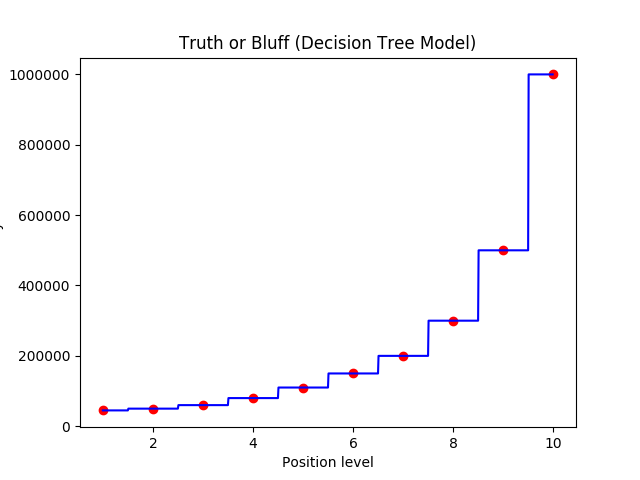
\includegraphics[scale=0.8]{pics/decision_tree}
\label{uloha1:pic1}
\caption{Decision Tree regression in Python} 
\end{center}
\end{figure}

\subsection{Random Forest Regression}
\textbf{Problem:} The same as in Polynomial regression.

Random Forest algorithm uses multiple Decision Trees and then average the results. Number of Decision Trees determines the number of splits and the value level of prediction.

The following code implements Random Forest Regressor in Python 

\lstinputlisting[style=Python, linerange=25-28]{code/random_forest_regression.py} 

The following code implements Random Forest Regressor in R 

\lstinputlisting[style=R, linerange=19-25]{code/random_forest_regression.R} 

\begin{figure}[H]
\centering
\begin{center}
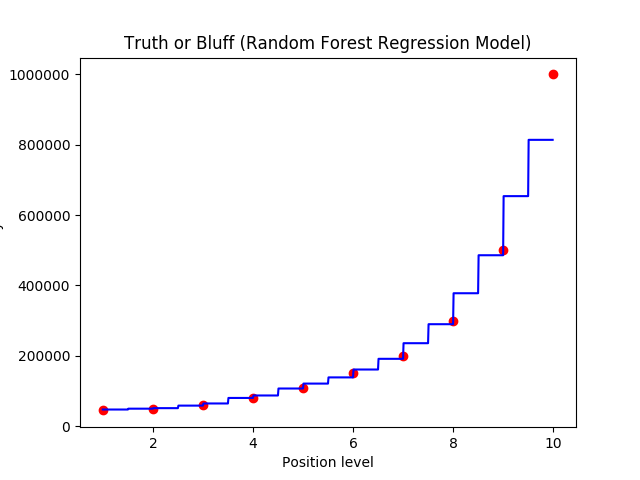
\includegraphics[scale=0.8]{pics/random_forest_python}
\label{uloha1:pic1}
\caption{Random Forest regression in Python} 
\end{center}
\end{figure}

\subsection{Evaluating model performance}

\subsubsection{R-squared}

$R^2$ - The Goodness of fit

\begin{equation}
R^2 = 1 - \frac{SS_{res}}{SS_{tot}}
\end{equation}

 $$SS_{res} = \sum_{0}^{n}(y_{i_{actual}} - y_{i_{predicted}})^2$$
 $$SS_{tot} = \sum_{0}^{n} (y_{i_{actual}} - y_{average})^2$$
 $SS_{res}$ means sum of squares residual and $SS_{tot}$ means sum of squares total, $n$ is the number of observations.
 
 The closer $R^2$ is to $1$, the better.

The biggest disadvantage is that $R^2$ never decrease if we introduce new independent variable to the model. That's why we use Adjusted $R^2$.

\subsubsection{Adjusted R-squared}
\begin{equation}
R^2_{adj} = 1-(1-R^2) \cdot \frac{n-1}{n-p-1}
\end{equation}

$ p ...$ number of regressors (independent variables), $ n ...$ sample size\\


\newpage
\section{Classification}

Classification is a statistical method which identifies a new observation into one of the several categories. More information here: \url{https://en.wikipedia.org/wiki/Statistical_classification}.

\textbf{Problem:} We will try to deal with the same problem for all listed methods below. We have a dataset of 400 users of some social network. The dataset tells us whether the user bought or didn't buy the product. The dataset contains user ID, salary and age. This is the sample of the dataset and the visualisation of the training set. Note that the axis shows values already scaled

\csvautotabular{csv/Social_Network_Ads.csv}


\begin{figure}[H]
\centering
\begin{center}
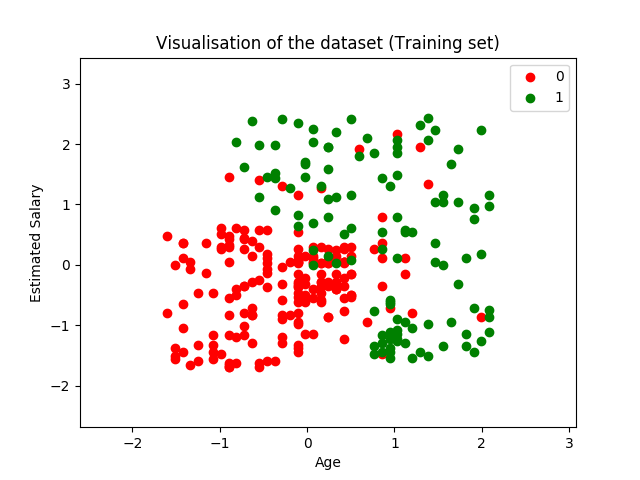
\includegraphics[scale=0.8]{pics/classification_dataset}
\label{uloha1:pic1}
\caption{Visualisation of the dataset for Classification problems. 1 means purchased, 0 means otherwise. Python} 
\end{center}
\end{figure}

\subsection{Classification code template in Python}
\lstset{basicstyle=\tiny}

\lstinputlisting[style=Python]{code/classification_template.py}

\subsection{Classification code template in R}

\lstinputlisting[style=R]{code/classification_template.R}


\subsection{Logistic regression}


Logistic regression deals with the situations when DV is in binary form (0/1, bought/didn't bought, etc.). The basic theory of Logistic regression is as follows: We take the Simple Linear Regression

\begin{equation}
y = b_0 + b_1*x_1,
\end{equation}

apply the \textit{Sigmoid function}

\begin{equation}
p = \frac{1}{1+e^{-y}}
\end{equation}

and solve 

\begin{equation}
ln(\frac{p}{1-p}) = b_0 + b_1*x_1.
\end{equation}

So basically this is what happens:

\begin{figure}[H]
\centering
\begin{center}
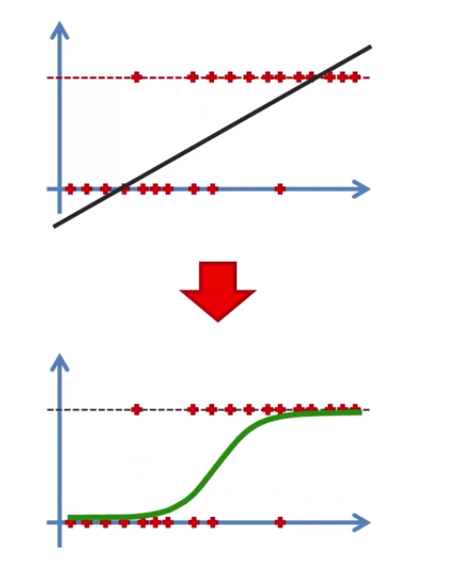
\includegraphics[scale=0.8]{pics/logistic_basic}
\label{uloha1:pic1}
\caption{Top - Simple Linear Regression, Bottom - Logistic Regression} 
\end{center}
\end{figure}

\lstset{basicstyle=\large}



This code implements Logistic regression in Python.
\lstinputlisting[style=Python, linerange=23-26]{code/logistic_regression.py} 


This code implements Logistic regression in R.
\lstinputlisting[style=R, linerange=22-25]{code/logistic_regression.R} 

\begin{figure}[H]
\centering
\begin{center}
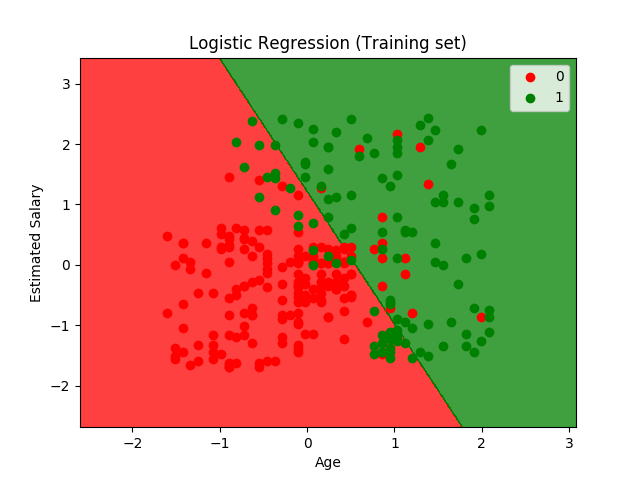
\includegraphics[scale=0.8]{pics/logistic}
\label{uloha1:pic1}
\caption{Logistic regression in Python} 
\end{center}
\end{figure}

\subsection{K-Nearest neighbours} 

K-Nearest neigbours works as follows: we take the new observation which we want to classify. Then we take a look at $k$ nearest points from the training set. Based on the nearest neighbours we decide the class of the new observation. We need to choose $k$ first. 

This code implements the K-NN classifier in Python.
\lstinputlisting[style=Python, linerange=23-27]{code/knn.py} 


This code implements the K-NN classifier in R.
\lstinputlisting[style=R, linerange=22-28]{code/knn.R} 

\begin{figure}[H]
\centering
\begin{center}
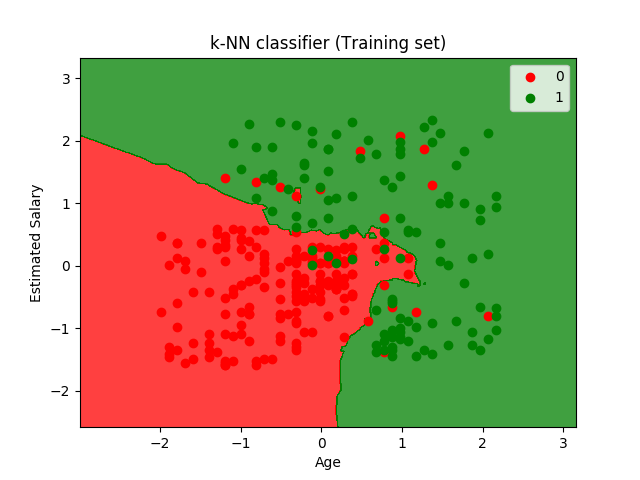
\includegraphics[scale=0.8]{pics/KNN}
\label{uloha1:pic1}
\caption{k-NN algorithm with $k=5$ in Python} 
\end{center}
\end{figure}

\subsection{SVM (Support Vector Machine)}

SVM classifier can be linear with linear kernel. SVM is \textbf{nonlinear} when using different kernel using the \textit{kernel trick} which maps the data to higher dimension to be linearly separable. More about SVM: \url{https://en.wikipedia.org/wiki/Support_vector_machine}. 

\begin{figure}[H]
\centering
\begin{center}
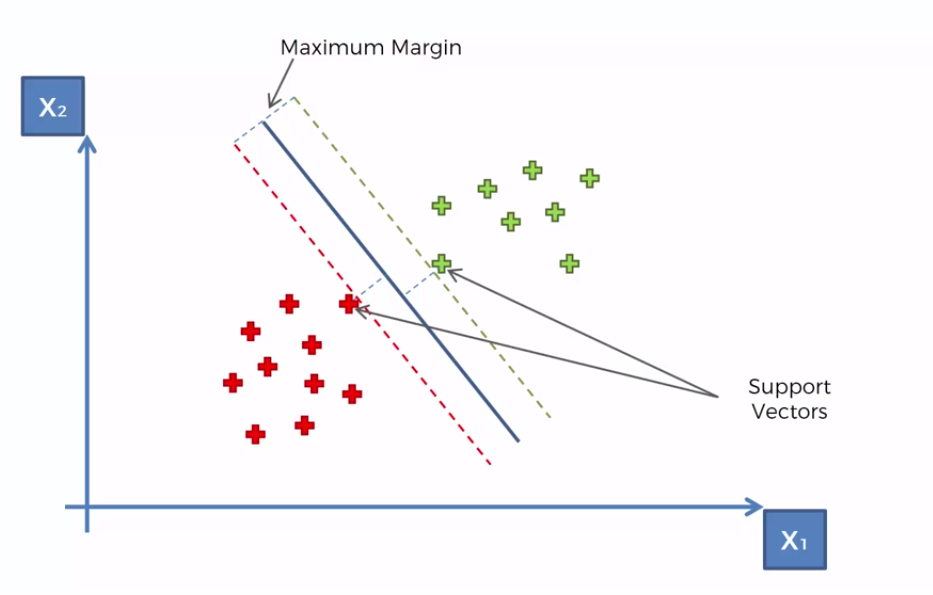
\includegraphics[scale=0.5]{pics/svm_basic}
\label{uloha1:pic1}
\caption{Support Vector Machine basic} 
\end{center}
\end{figure}

This code implements the SVM classifier in Python.
\lstinputlisting[style=Python, linerange=23-26]{code/svm.py} 


This code implements the SVM classifier in R.
\lstinputlisting[style=R, linerange=22-28]{code/svm.R} 

\begin{figure}[H]
\centering
\begin{center}
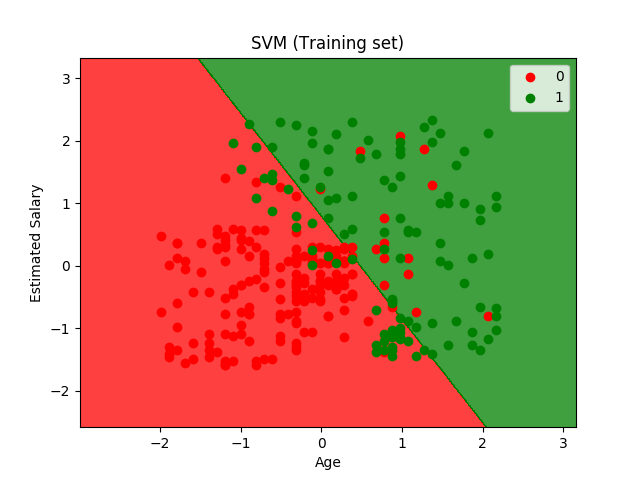
\includegraphics[scale=0.8]{pics/svm_linear}
\label{uloha1:pic1}
\caption{Support Vector Machine with \textbf{linear} kernel in Python} 
\end{center}
\end{figure}

\begin{figure}[H]
\centering
\begin{center}
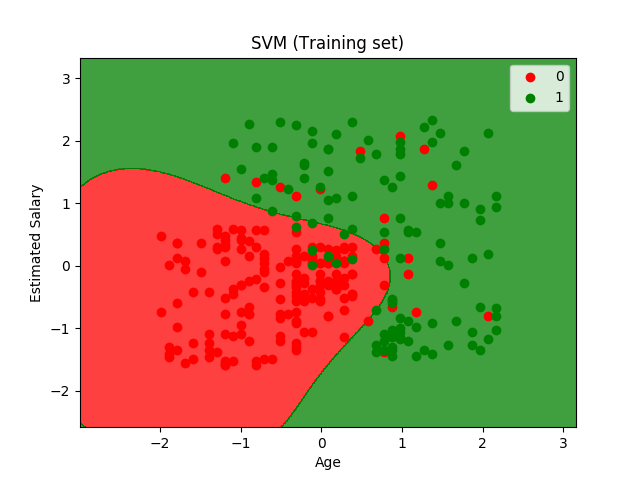
\includegraphics[scale=0.8]{pics/svm}
\label{uloha1:pic1}
\caption{Support Vector Machine with \textbf{RBF} kernel in Python} 
\end{center}
\end{figure}

\subsection{Kernel SVM}

More about Kernel SVM in the Udemy course.

\subsection{Naive Bayes}


The Bayes theorem is the known equation: 
\begin{equation}
P(A|X) = \frac{P(X|A) \cdot P(A)}{P(X)}.
\end{equation}

$A$ is the DV and can have two values $a_1; a_2$ and $X$ is the feature vector. 

In Naive Bayes Classification method we calculate the variables in the equation in this order:

\begin{enumerate}
\item $P(A)= \frac{\text{number of observations with property-} a_i}{\text{number of total observations}}$ ... prior probability. 
\item $P(X) = \frac{\text{number of similar observations}}{\text{number of total observations}}$ ... marginal likelihood. Probabilty of the occurence of the particular combination of feature vector $X$. Number of similar observations depends on the are we define.
\item $P(X|A) = \frac{\text{number of similar observations with property-} a_i}{\text{number of total observations with property-} a_i}$ ... likelihood. 
\item $P(A|X)$ ... finally we get posterior probabily which we were looking for.
\end{enumerate}

This code implements the Naive Bayes Classifier in Python.
\lstinputlisting[style=Python, linerange=23-26]{code/naive_bayes.py} 


This code implements the Naive Bayes Classifier in R.
\lstinputlisting[style=R, linerange=22-26]{code/naive_bayes.R} 


\begin{figure}[H]
\centering
\begin{center}
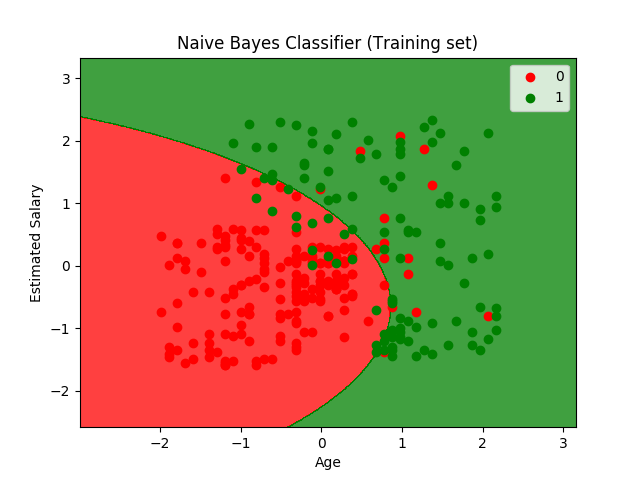
\includegraphics[scale=0.8]{pics/bayes}
\label{uloha1:pic1}
\caption{Naive Bayes Classifier in Python} 
\end{center}
\end{figure}

\subsection{Decision Tree Classification}

Term \textbf{CART} - Classification and Regression Trees.

Similar to Decision Tree Regression.  

This code implements the Decision Tree Classifier in Python.
\lstinputlisting[style=Python, linerange=23-26]{code/decision_tree_classification.py} 


This code implements the Decision Tree Classifier in R.
\lstinputlisting[style=R, linerange=22-26]{code/decision_tree_classification.R} 

\begin{figure}[H]
\centering
\begin{center}
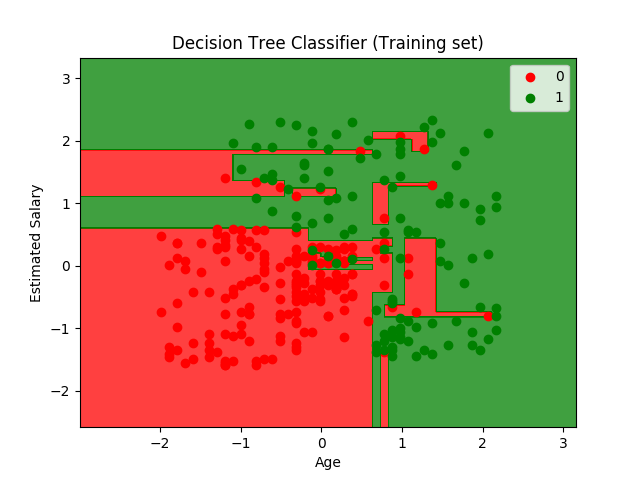
\includegraphics[scale=0.8]{pics/dtc}
\label{uloha1:pic1}
\caption{Decision Tree in Python} 
\end{center}
\end{figure}

In R we can also see the Decision Tree itself simply by using \verb|plot(classifier)|. 

\begin{figure}[H]
\centering
\begin{center}
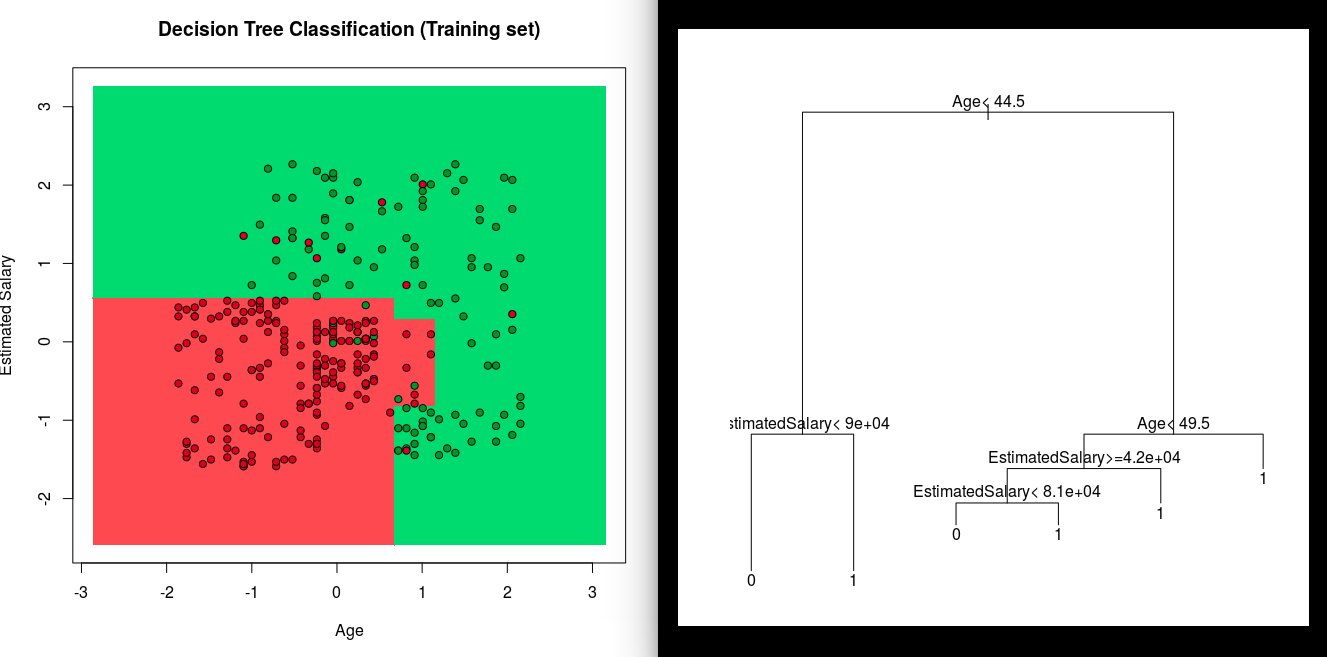
\includegraphics[scale=0.33]{pics/dtr}
\label{uloha1:pic1}
\caption{Decision Tree in R. Visualisation and Decision Tree itself} 
\end{center}
\end{figure}

\subsection{Random Forest Classification}

Similarly to Random Forest Regression, the Random Forest Classification uses many Decision Trees and then average their results. Random Forest Classification is the algorithm of choice for the Microsoft Kinect developers.

This code implements the Decision Tree Classifier in Python.
\lstinputlisting[style=Python, linerange=23-27]{code/random_forest_classification.py} 


This code implements the Decision Tree Classifier in R.
\lstinputlisting[style=R, linerange=22-28]{code/random_forest_classification.R} 

\begin{figure}[H]
\centering
\begin{center}
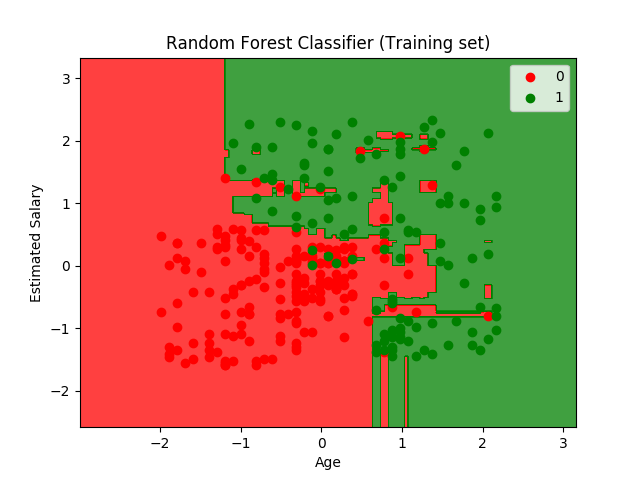
\includegraphics[scale=0.8]{pics/rfc}
\label{uloha1:pic1}
\caption{Random Forest Classifier with 10 Decision Trees in Python} 
\end{center}
\end{figure}

\subsection{Evaluating Classification model performance}

The following approaches are used to pick the best model.

\subsubsection{Confusion matrix}

Confusion matrix tells us number of Correct predictions (sum of diagonal) and number of wrong predictions. It also distinguish 
\begin{itemize}
\item Type error 1 (False positive)
\item Type error 2 (False negative).
\end{itemize}  

\begin{figure}[H]
\centering
\begin{center}
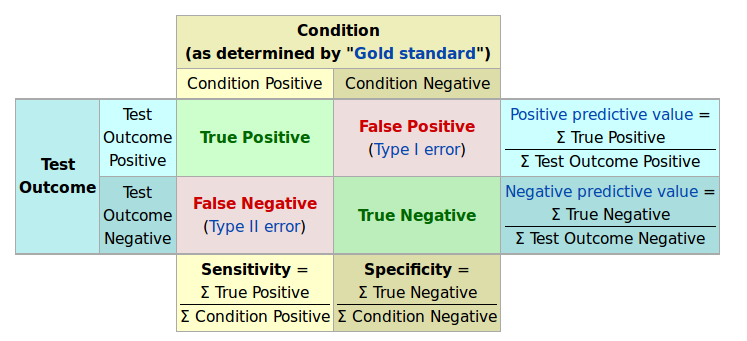
\includegraphics[scale=0.5]{pics/cm}
\label{uloha1:pic1}
\caption{Confusion matrix} 
\end{center}
\end{figure}


\subsubsection{Accuracy paradox}
Unfortunately the confusion matrix has one big withdrawal. Let's define Accuracy rate.

\begin{equation}
AR = \frac{n_{correct}}{n_{total}}
\end{equation}

It should not be considered the ultimate measure for the performance of the models. Let's consider the following scenario. We build a model with the following confusion matrix:

% \usepackage{multirow}
\begin{table}[H]
\centering
\caption{Situation before}
\label{my-label}
\begin{tabular}{|l|l|l|l|}
\hline
                           & \multicolumn{3}{l|}{Predicted DV} \\ \hline
\multirow{3}{*}{Actual DV} &          & 0          & 1         \\ \cline{2-4} 
                           & 0        & 9700       & 150       \\ \cline{2-4} 
                           & 1        & 50         & 100       \\ \hline
\end{tabular}
\end{table}

We simply calculate that the Accuracy rate is $AR = 9800/10000 = 98\%$. Then we abandon the model and always predict negative (0). We come out with the following confusion matrix.

\begin{table}[H]
\centering
\caption{Situation without model but with better AR}
\label{my-label}
\begin{tabular}{|l|l|l|l|}
\hline
                           & \multicolumn{3}{l|}{Predicted DV} \\ \hline
\multirow{3}{*}{Actual DV} &          & 0           & 1        \\ \cline{2-4} 
                           & 0        & 9850        & 0        \\ \cline{2-4} 
                           & 1        & 150         & 0        \\ \hline
\end{tabular}
\end{table}

We calculate that the Accuracy rate is $AR = 9850/10000 = 98.5\%$. We have three times more Type 2 errors but the AR is better. That's why \textbf{Accuracy rate is not the best evaluating technique!}


\subsubsection{CAP curve}

\textbf{CAP} stands for Cumulative Accuracy Profile. 

\textbf{Problem:} We have a dataset of 100000 customers and 10\% of them will purchase the product. We want to build a model which finds the customers with the highest probability of purchasing the product. Then we contact them. We want our model to have the highest possible hit rate of contacted-purchased. The "Crystal ball" will have 100\% hit rate, that means first 10000 contacted equeals 10000 purchases.

\begin{figure}[H]
\centering
\begin{center}
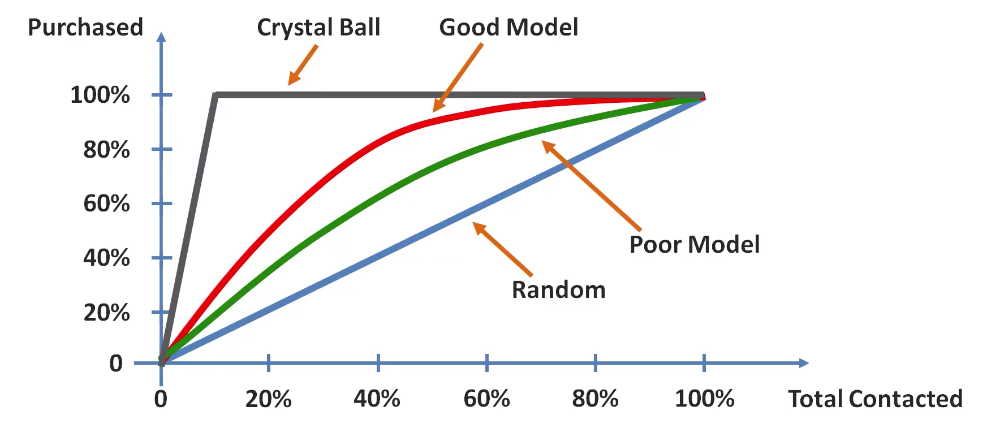
\includegraphics[scale=0.4]{pics/cap}
\label{uloha1:pic1}
\caption{CAP curve explained} 
\end{center}
\end{figure}


\newpage
\section{Clustering}

Clustering is the form of unsupervised learning. That means we do not have a training set but we have to find the clusters ourselves. We will show two approches. The first step in both of them is to establish the number of clusters $k$. Each approach use different method.

\textbf{Problem:} We are data analysts hired by mall company. They provide us with the dataset containing information about their customers. They want us to divide their customers into several (not specified $k$) classes. This is the sample of the dataset. We will use only \textit{salary} and \textit{spending score}.

\csvautotabular{csv/Mall_Customers.csv}


\begin{figure}[H]
\centering
\begin{center}
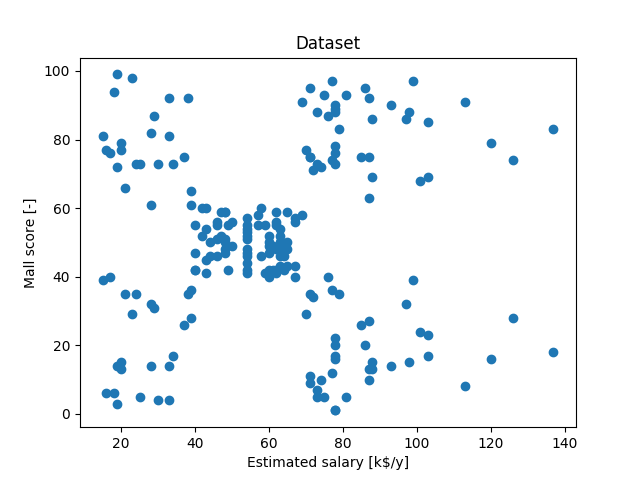
\includegraphics[scale=0.8]{pics/k_means_data}
\label{uloha1:pic1}
\caption{Visualisation of the dataset for clustering problem in Python} 
\end{center}
\end{figure}

\subsection{K-means clustering}

\begin{enumerate}
\item Choose the number $k$ of clusters.
\item Select at random $k$ points. The \textit{centroids}. (not necessarily from the dataset)
\item Assign each datapoint to the closest \textit{centroid}, that forms $k$ clusters.
\item Compute and place the new \textit{centroids} for each cluster.
\item Reassing each point according to the new \textit{centroids} and go to step 4. If no reassignment took place. \textbf{Your model is ready}.
\end{enumerate}

\bigskip

Selecting the random points for \textit{centroids} might be problematic and can lead to faulty results. K-means++ algorithm deals with it.

\subsubsection{Elbow method to find optimal K}

First of all we need to establish the number of clustes $k$. In K-means we use the "Elbow method".


We place a \textit{Centroid} in the dataset and calculate the distances between all the points and the centroid. Then we place another \textit{centroid} and calculate and sum the distances of all points to the closest \textit{centrois}. We will call this value \textit{WCSS} We continue to increase the number of \textit{centroids} $k$. It is clear that as $k$ closes to the number of the points in the dataset, the \textit{WCSS} gets closer to zero. 

The equation can be written as 

\begin{equation}
WCSS = \sum_{1}^{k} (\sum_{P_i \text{in Cluster i}} dist(P_i, C_1)^2)
\end{equation}

where $k$ is the number of clusters. We can plot the values in the graph and choose the $k$ from the "elbow".

\begin{figure}[H]
\centering
\begin{center}
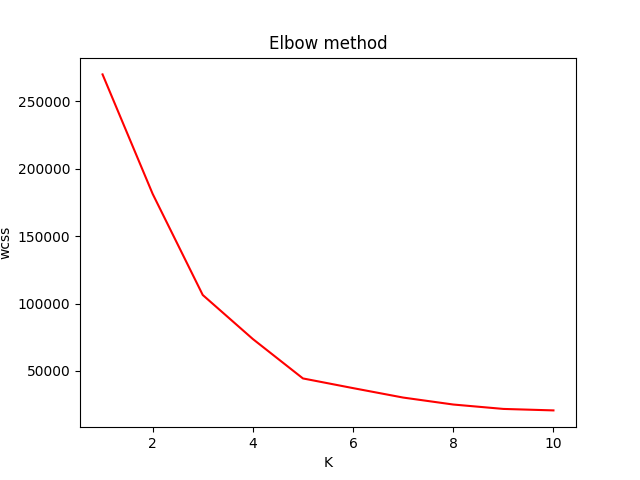
\includegraphics[scale=0.8]{pics/elbow}
\label{uloha1:pic1}
\caption{Elbow method to determine the optimal K in Python} 
\end{center}
\end{figure}

From the picture we see that the optimal $k$ is 5.


\subsubsection{Implementation}

\lstset{basicstyle=\tiny}
This code implements the K-means algorithm in Python with the elbow method and visualisation.
\lstinputlisting[style=Python]{code/kmeans.py} 


This code implements the K-means algorithm in R with the elbow method and visualisation.
\lstinputlisting[style=R]{code/kmeans.R} 


\begin{figure}[H]
\centering
\begin{center}
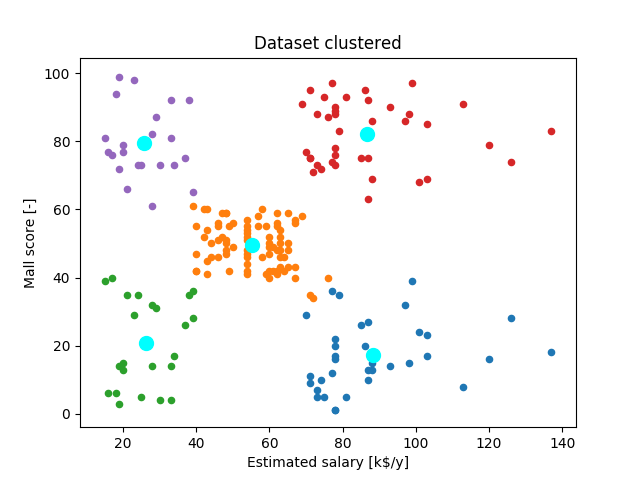
\includegraphics[scale=0.8]{pics/k_means}
\label{uloha1:pic1}
\caption{Result of K-mean algorithm in Python, blue points are centroids.} 
\end{center}
\end{figure}


\subsection{Hierarchical clustering}

Agglomerative HC:
\begin{enumerate}
\item Make each data point a single cluster (that makes N clusters)
\item Take the two closest points and make them 1 cluster (N-1 clusters)
\item Take the two \textbf{closest clusters} and make them 1 cluster (N-2 clusters)
\item Repeat step 3 until there is only 1 cluster 
\end{enumerate}

What is the \textbf{distance between clusters}? We have several valid answers. It depends on the usecase.

\begin{itemize}
\item Distance of closest points
\item Distance of furthest points
\item Average distance
\item Distance of centroids
\end{itemize}

\subsubsection{Dendrograms}

To choose the optimal $k$ - the number of clusters, we use dendrograms. Dendrograms trace the history of points clustering and their distances (or disimilarities). We choose the longest vertical line that can be split by horizontal line without interruption.

\begin{figure}[H]
\centering
\begin{center}
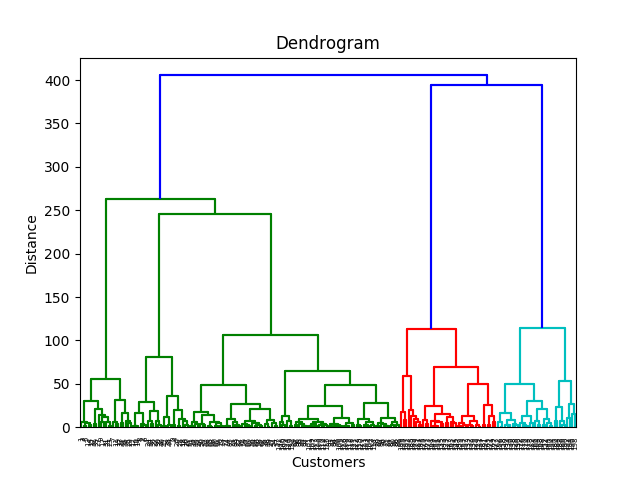
\includegraphics[scale=0.8]{pics/hc_dendrogram}
\label{uloha1:pic1}
\caption{Dendrogram - scipy library in Python} 
\end{center}
\end{figure}

Code

linkage is the method that is trying to minimize the variance in each cluser.

\begin{figure}[H]
\centering
\begin{center}
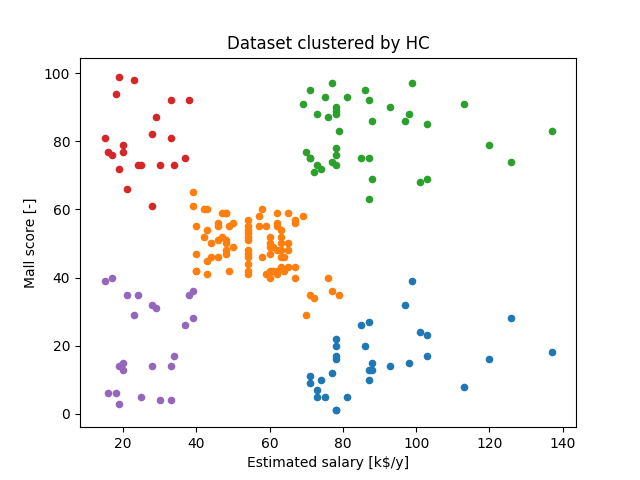
\includegraphics[scale=0.8]{pics/hc}
\label{uloha1:pic1}
\caption{Result of hierarchical clustering in Python} 
\end{center}
\end{figure}




\newpage

\section{Association rule learning}

\textit{"People who bought ... also bought ..."}

\textbf{Problem:}We have a dataset containing transactions in a mall. We want to find associative rules. Here is the sample of the dataset. One row is one basket bought in the mall. 


\csvautotabular{csv/Market_Basket_Optimisation.csv}


\subsection{Apriori}

The important variables. The examples are from the problem.

\begin{itemize}
\item Support (M1) $= \frac{  transactions \text{\space} containing \text{\space} M1}{  total  \text{\space} transactions}$
\item Confidence (M1 $\rightarrow$ M2) = $\frac{transactions  \text{\space} containing \text{\space} M1  \text{\space}and \text{\space}M2}{transactions \text{\space} containing \text{\space}M1}$
\item Lift (M1 $\rightarrow$ M2) = $\frac{Confidence(M1 \rightarrow M2)}{Support(M2)}$
\end{itemize}

\bigskip

The algorithm has following steps:
\begin{enumerate}
\item Select a minimum support and confidence.
\item Take all the subsets in transactions having higher support than minimum support.
\item Take all the rules of these subsets having higher confidence than minimum confidence.
\item Sort the rules by decreasing lift.
\end{enumerate}

\lstset{basicstyle=\tiny}
This code implements the Apriori algorithm in R.
\lstinputlisting[style=Python]{code/apriori.R} 

\begin{figure}[H]
\centering
\begin{center}
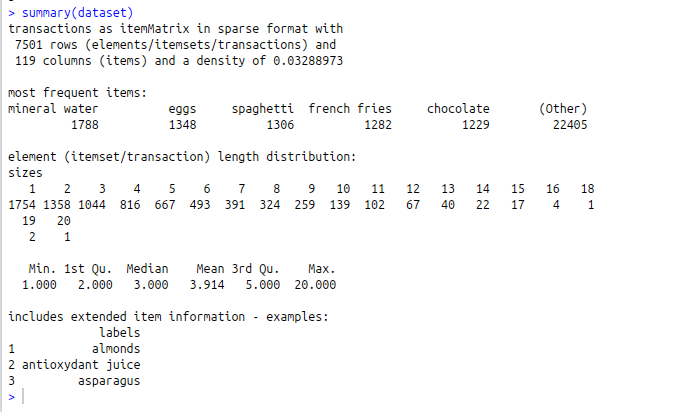
\includegraphics[scale=0.6]{pics/apriori_data}
\label{uloha1:pic1}
\caption{Summary of the R object. It is the matrix with a small amount of "ones" and a lot of "zeros". The number of rows equals the number of transactions and number of columns equals the cardinality of bought items set} 
\end{center}
\end{figure}

\begin{figure}[H]
\centering
\begin{center}
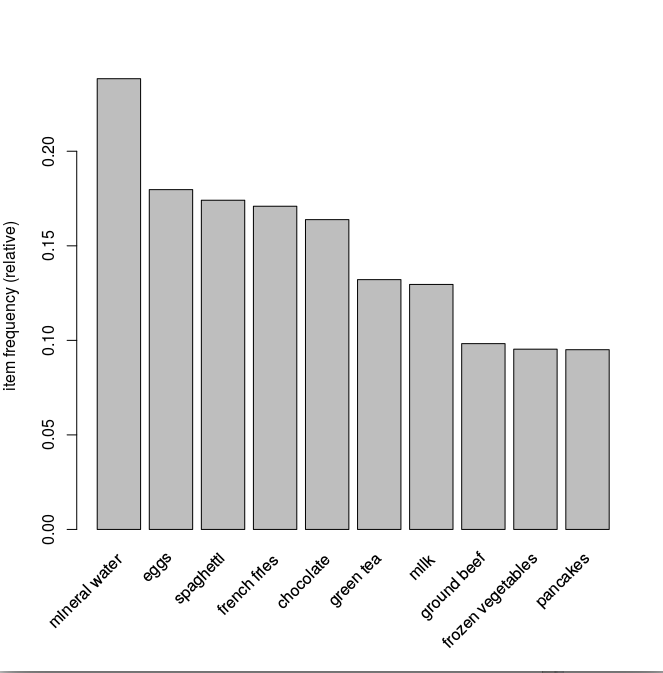
\includegraphics[scale=0.6]{pics/apriori_support}
\label{uloha1:pic1}
\caption{Visualisation of the most bought products. That means it shows their support} 
\end{center}
\end{figure}


\begin{figure}[H]
\centering
\begin{center}
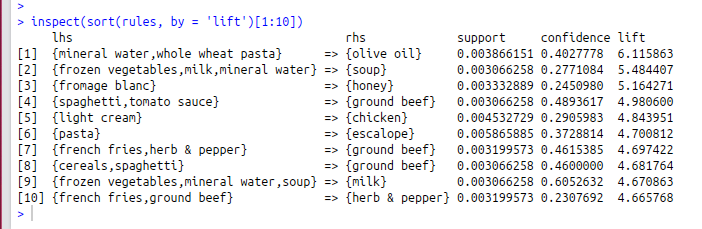
\includegraphics[scale=0.6]{pics/apriori_result}
\label{uloha1:pic1}
\caption{Top 10 found rules in the dataset of bascet. Sorted by lift} 
\end{center}
\end{figure}

\subsection{Eclat}



Eclat is similar to Apriori but much easier. We use only support.

The algorithm has following steps:
\begin{enumerate}
\item Select a minimum support.
\item Take all the subsets in transactions having higher support than minimum support.
\item Sort these subsets by decreasing support.
\end{enumerate}

This code implements the Eclat algorithm in R. The only differences between this and Apriori is the function call and only support parameter.

\lstset{basicstyle=\large}
\lstinputlisting[style=R, linerange=10-13]{code/eclat.R} 

\newpage

\section{Reinforcement learning}

Reinforcement Learning is a branch of Machine Learning, also called Online Learning. It is used to solve interacting problems where the data observed up to time $t$ is considered to decide which action to take at time $t + 1$. It is also used for Artificial Intelligence when training machines to perform tasks such as walking. Desired outcomes provide the AI with reward, undesired with punishment. Machines learn through trial and error.

\subsection{Upper Confidence Bound (UCB)}


\subsection{Thompson sampling}
We are creating probabilistic view.

\newpage

\section{Natural language processing}
Natural Language Processing (or NLP) is applying Machine Learning models to text and language. Teaching machines to understand what is said in spoken and written word is the focus of Natural Language Processing. Whenever you dictate something into your iPhone / Android device that is then converted to text, that’s an NLP algorithm in action.

You can also use NLP on a text review to predict if the review is a good one or a bad one. You can use NLP on an article to predict some categories of the articles you are trying to segment. You can use NLP on a book to predict the genre of the book. And it can go further, you can use NLP to build a machine translator or a speech recognition system, and in that last example you use classification algorithms to classify language. Speaking of classification algorithms, most of NLP algorithms are classification models, and they include Logistic Regression, Naive Bayes, CART which is a model based on decision trees, Maximum Entropy again related to Decision Trees, Hidden Markov Models which are models based on Markov processes.

A very well-known model in NLP is the Bag of Words model. It is a model used to preprocess the texts to classify before fitting the classification algorithms on the observations containing the texts.

In this part, you will understand and learn how to:

\begin{itemize}
\item Clean texts to prepare them for the Machine Learning models,
\item Create a Bag of Words model,
\item Apply Machine Learning models onto this Bag of Worlds model.
\end{itemize}


\newpage
\section{Deep learning}

Deep Learning is the most exciting and powerful branch of Machine Learning. Deep Learning models can be used for a variety of complex tasks:

\begin{itemize}
\item Artificial Neural Networks for Regression and Classification
\item Convolutional Neural Networks for Computer Vision
\item Recurrent Neural Networks for Time Series Analysis
\item Self Organizing Maps for Feature Extraction
\item Deep Boltzmann Machines for Recommendation Systems
\item Auto Encoders for Recommendation Systems
\end{itemize}

In this part, you will understand and learn how to implement the following Deep Learning models:
\begin{enumerate}
\item Artificial Neural Networks for a Business Problem
\item Convolutional Neural Networks for a Computer Vision task
\end{enumerate}

\subsection{Artificial Neural Network}
\subsection{Convolutional Neural Network}

\newpage

\section{Dimensionality reduction}
\subsection{Principal Component Analysis (PCA)}
\subsection{Linear Discriminant Analysis (LDA)}
\subsection{Kernel PCA}

\newpage

\section{Model selection and boosting}
\subsection{Model selection}
\subsection{XGBoost}

\bibliography{references}
\nocite{*} 

\end{document}
